\chapter{The NED Language}
\label{cha:the-ned-language}


\section{NED overview}

The user describes the structure of a simulation model in the NED language. NED
stands for Network Description. NED lets the user declare simple modules, and
connect and assemble them into compound modules. The user can label some compound
modules as \textit{networks}, self-contained simulation models. Channels are
another component type, whose instances can also be used in compound modules.

The NED language has several features which let it scale well to large projects:

\begin{description}

\item[Hierarchical] The traditional way to deal with complexity is via
introducing hierarchies. In {\opp}, any module which would be too complex as
a single entity can be broken down into smaller modules, and used as a
compound module.

\item[Component-Based] Simple modules and compound modules are inherently
reusable, which not only reduces code copying, but more importantly, allows
component libraries (like the INET Framework, MiXiM, Castalia, etc.) to
exist.

\item[Interfaces] Module and channel interfaces can be used as a
placeholder where normally a module or channel type would be used, and the
concrete module or channel type is determined at network setup time by a
parameter. Concrete module types have to ``implement'' the interface they
can substitute. For example, given a compound module type named
\ttt{MobileHost} contains a \ttt{mobility} submodule of the type
\ttt{IMobility} (where \ttt{IMobility} is a module interface), the actual
type of \ttt{mobility} may be chosen from the module types that implemented
\ttt{IMobility} (\ttt{RandomWalkMobility}, \ttt{TurtleMobility}, etc.)

\item[Inheritance] Modules and channels can be subclassed. Derived modules
and channels may add new parameters, gates, and (in the case of compound
modules) new submodules and connections. They may set existing parameters
to a specific value, and also set the gate size of a gate vector. This
makes it possible, for example, to take a \ttt{GenericTCPClientApp} module
and derive an \ttt{FTPClientApp} from it by setting certain parameters to a fixed
value; or to derive a \ttt{WebClientHost} compound module from a
\ttt{BaseHost} compound module by adding a \ttt{WebClientApp} submodule and
connecting it to the inherited \ttt{TCP} submodule.

\item[Packages] The NED language features a Java-like package structure,
to reduce the risk of name clashes between different models. \ttt{NEDPATH}
(similar to Java's \ttt{CLASSPATH}) was also introduced to make it easier
to specify dependencies among simulation models.

\item[Inner types] Channel types and module types used locally by a
compound module can be defined within the compound module, in order to
reduce namespace pollution.

\item[Metadata annotations] It is possible to annotate module or channel
types, parameters, gates and submodules by adding properties. Metadata are
not used by the simulation kernel directly, but they can carry extra
information for various tools, the runtime environment, or even for other
modules in the model. For example, a module's graphical representation
(icon, etc)  or the prompt string and measurement unit (milliwatt, etc) of a
parameter are already specified as metadata annotations.

\end{description}

\begin{note}
    The NED language has changed significantly in the 4.0 version.
    Inheritance, interfaces, packages, inner types, metadata annotations, inout
    gates were all added in the 4.0 release, together with many other features.
    Since the basic syntax has changed as well, old NED files need to be
    converted to the new syntax. There are automated tools for this purpose, so
    manual editing is only needed to take advantage of new NED features.
\end{note}

The NED language has an equivalent tree representation which can be
serialized to XML; that is, NED files can be converted to XML and back
without loss of data, including comments. This lowers the barrier for
programmatic manipulation of NED files, for example extracting information,
refactoring and transforming NED, generating NED from information stored in
other system like SQL databases, and so on.

\begin{note}
    This chapter is going to explain the NED language gradually, via examples.
    If you are looking for a more formal and concise treatment, see
    Appendix \ref{cha:ned-language-grammar}.
\end{note}


\section{Warmup}

In this section we introduce the NED language via a complete and
reasonably real-life example: a communication network.

Our hypothetical network consists of nodes. One each node there's an
application running which generates packets at random intervals.
The nodes are routers themselves as well. We assume that the application
uses datagram-based communication, so that we can leave out the
transport layer from the model.

%% XXX keep the example simple!

\subsection{The network}

First we'll define the network, then in the next sections we'll continue
to define the network nodes.

Let the network topology be as in Figure \ref{fig:ned-net6-topology}.

\begin{figure}[htbp]
  \begin{center}
    \includegraphics[scale=0.6]{figures/ned-net6-topology}
    \caption{The network}
    \label{fig:ned-net6-topology}
  \end{center}
\end{figure}

The corresponding NED description would look like this:

\begin{Verbatim}
//
// A six-node network
//
network Net6
{
    submodules:
        node1: Node;
        node2: Node;
        node3: Node;
        node4: Node;
        node5: Node;
        node6: Node;
    connections:
        node1.port++ <--> {datarate=100Mbps;} <--> node2.port++;
        node2.port++ <--> {datarate=100Mbps;} <--> node4.port++;
        node4.port++ <--> {datarate=100Mbps;} <--> node6.port++;
        ...
        node3.port++ <--> {datarate=100Mbps;} <--> node4.port++;
}
\end{Verbatim}

The above code defines a network type named \ttt{Net6}. Note that the NED
language uses the familiar curly brace syntax, and ``\ttt{//}'' to denote
comments.

\begin{note}
    Comments in NED not only make the source code more readable, but in the
    {\opp} IDE they also get displayed at various places (tooltips, content
    assist, etc), and become part of the documentation extracted from the NED
    files. The NED documentation system, not unlike \textit{JavaDoc} or
    \textit{Doxygen}, will be described in Chapter \ref{cha:neddoc}.
\end{note}

The network contains six nodes, named \ttt{node1}...\ttt{node6},
from the NED module type \ttt{Node}. (We'll define \ttt{Node} in the next
sections.)

The second half of the declaration defines how the nodes are to be
connected. The double arrow means bidirectional connection. The connection
points of modules are called gates, and the \ttt{port++} notation adds a
new gate to the \ttt{port[]} gate vector. Gates and connections will be
covered in more detail in sections XXX and XXX. Nodes are connected
with a channel that has a data rate of 100Mbps.

\begin{note}
    In many other systems, the equivalent of {\opp} gates are called
    \textit{ports}. We have retained the term \textit{gate} to reduce
    collisions with other uses of the otherwise overloaded word
    \textit{port}: router port, TCP port, I/O port, etc.
\end{note}

The above code would be placed into a file named \ttt{Net6.ned}. It is
a convention to put every NED definition into its own file and to name the
file accordingly, but it is not mandatory to do so.

One can define any number of networks in the NED files, and for every
simulation the user has to specify which network he wants to set up.
The usual way of specifying the network is to put the \fconfig{network}
option into the configuration (by default the \ttt{omnetpp.ini} file):

\begin{Verbatim}
[General]
network = Net6
\end{Verbatim}


\subsection{Introducing a channel}

It is cumbersome to have to repeat the data rate for every connection.
Luckily, NED provides a convenient solution: one can create a new channel
type that encapsulates the data rate setting, and this channel type can
be defined inside the network so that it does not litter the global
namespace.

The improved network will look like this:

\begin{Verbatim}
//
// A six-node network
//
network Net6
{
    types:
        channel C extends ned.DatarateChannel {
            datarate = 100Mbps;
        }
    submodules:
        node1: Node;
        node2: Node;
        node3: Node;
        node4: Node;
        node5: Node;
        node6: Node;
    connections:
        node1.port++ <--> C <--> node2.port++;
        node2.port++ <--> C <--> node4.port++;
        node4.port++ <--> C <--> node6.port++;
        ...
        node3.port++ <--> C <--> node4.port++;
}
\end{Verbatim}

Later sections will cover the concepts used (inner types, channels, the
\ttt{DatarateChannel} built-in type, inheritance) in details.


\subsection{The App, Routing and Queue simple modules}

Simple modules are the basic building blocks for other (compound) modules.
All active behavior in the model is encapsulated in simple modules.
Behavior is defined with a C++ class; NED files only declare the externally
visible interface of the module (gates, parameters).

In our example, we could define \ttt{Node} as a simple module. However,
its functionality is quite complex (traffic generation, routing, etc),
so it is better to implement it with several smaller simple module types
which we are going to assemble into a compound module. We'll have
one simple module for traffic generation (\ttt{App}), one for routing
(\ttt{Routing}), and one for queueing up packets to be sent out (\ttt{Queue}).
For brevity, we omit the bodies of the latter two in the code below.

\begin{Verbatim}[commandchars=\\\{\}]
simple App
\{
    parameters:
        int destAddress;
        ...
        @display("i=block/browser");
    gates:
        input in;
        output out;
\}

simple Routing
\{
    ...
\}

simple Queue
\{
    ...
\}
\end{Verbatim}

By convention, the above simple module declarations go into the
\ttt{App.ned}, \ttt{Routing.ned} and \ttt{Queue.ned} files.

\begin{note}
    Note that module type names (\ttt{App}, \ttt{Routing}, \ttt{Queue})
    begin with a capital letter, and parameter and gate names begin with
    lowercase -- this is the recommended naming convention. Capitalization
    matters because the language is case sensitive.
\end{note}

Let us see the first simple module type declaration. \ttt{App} has a
parameter called \ttt{destAddress} (others have been omitted for now),
and two gates named \ttt{out} and \ttt{in} for sending and receiving
application packets.

The argument of \ttt{@display()} is called a \textit{display string},
and it defines the default rendering of the module in graphical environments;
\ttt{"i=..."} defines the default icon.

Generally, \ttt{@}-words like \ttt{@display} are called \textit{properties}
in NED, and they are used to annotate various objects
with metadata. Properties can be attached to files, modules, parameters, gates,
connections, and other objects, and parameter values have a very flexible
syntax.


\subsection{The Node compound module}

Now we can assemble \ttt{App}, \ttt{Routing} and {Queue} into the
compound module \ttt{Node}. A compound module can be thought of as
a ``cardboard box'' that groups other modules into a larger unit,
which can further be used as a building block for other modules;
networks are also a kind of compound module.

\begin{Verbatim}[commandchars=\\\{\}]
module Node
\{
    parameters:
        @display("i=misc/node_vs,gold");
    gates:
        inout port[];
    submodules:
        app: App;
        routing: Routing;
        queue[sizeof(port)]: Queue;
    connections:
        routing.localOut --> app.in;
        routing.localIn <-- app.out;
        for i=0..sizeof(port)-1 \{
            routing.out[i] --> queue[i].in;
            routing.in[i] <-- queue[i].out;
            queue[i].line <--> port[i];
        \}
\}
\end{Verbatim}

Compound modules, like simple modules, may have parameters and gates.
Our \ttt{Node} module contains an \ttt{address} parameter, plus a
\textit{gate vector} of unspecified size, named \ttt{port}.
The actual gate vector size will be determined implicitly by the number
of neighbours when we create a network from nodes of this type.
The type of \ttt{port[]} is \ttt{inout}, which allows bidirectional
connections.

The modules that make up the compound module are listed under \ttt{submodules}.
Our \ttt{Node} compound module type has an \ttt{app} and a \ttt{routing}
\textit{submodule}, plus a \ttt{queue[]} \textit{submodule vector} that
contains one \ttt{Queue} module for each port, as specified by
\ttt{[sizeof(port)]}.

XXX explain "for" loop

\subsection{Putting it together}

XXX Explain how the network is set up! top-down etc

\bigskip
\begin{center}* * *\end{center}
\bigskip

In the following sections we'll go through the elements of the NED
language and look at them in more details.



\section{Simple modules}

Simple modules are the active components in the model.
Simple modules are defined with the \fkeyword{simple} keyword.

An example simple module:

\begin{Verbatim}[commandchars=\\\{\}]
simple Queue
\{
    parameters:
        int capacity;
        @display("i=block/queue");
    gates:
        input in;
        output out;
\}
\end{Verbatim}

Both the \fkeyword{parameters} and \fkeyword{gates} sections are optional, that is,
they can be left out if there's no parameter or gate. In addition, the
\fkeyword{parameters} keyword itself is optional too, it can be left out
even if there are parameters or properties.

Note that the NED definition doesn't contain any code to define the
operation of the module: that part is expressed in C++. By default, {\opp}
looks for C++ classes of the same name as the NED type (so here, \ttt{Queue}).

One can explicitly specify the C++ class with the \ttt{@class} property.
Classes with namespace qualifiers are also accepted, as shown in the following
example that uses the \ttt{mylib::Queue} class:

\begin{Verbatim}[commandchars=\\\{\}]
simple Queue
\{
    parameters:
        int capacity;
        @class(mylib::Queue);
        @display("i=block/queue");
    gates:
        input in;
        output out;
\}
\end{Verbatim}

If you have several modules that are all in a common namespace, then a
better alternative to \ttt{@class} is the \ttt{@namespace} property. The
C++ namespace given with \ttt{@namespace} will be prepended to the normal
class name. In the following example, the C++ classes will be
\ttt{mylib::App}, \ttt{mylib::Router} and \ttt{mylib::Queue}:

\begin{Verbatim}
@namespace(mylib);

simple App {
   ...
}

simple Router {
   ...
}

simple Queue {
   ...
}
\end{Verbatim}

As you've seen, \ttt{@namespace} can be specified on file level. Moreover,
when placed in a file called \ttt{package.ned}, the namespace will apply to
all files in the same directory and all directories below.

The implementation C++ classes need to be subclassed from the
\cclass{cSimpleModule} library class; chapter XXX of this manual describes
in detail how to write them.

Simple modules can be extended (or specialized) via subclassing.
The motivation for subclassing can be to set some open parameters
or gate sizes to a fixed value (see XXX), or to replace the C++
class with a different one. Now, by default the derived NED module type
will \textit{inherit} the C++ class from its base, so it is important
to remember that you need to write out \ttt{@class} if you want it
to use the new class.

The following example shows how to specialize a module by setting a parameter
to a fixed value (and leaving the C++ class unchanged):

\begin{Verbatim}
simple Queue
{
   int capacity;
   ...
}

simple BoundedQueue extends Queue
{
   capacity = 10;
}
\end{Verbatim}

In the next example, the author wrote a \ttt{PriorityQueue} C++ class, and
wants to have a corresponding NED type, derived from \ttt{Queue}. However,
it does not work as expected:

\begin{Verbatim}
simple PriorityQueue extends Queue // wrong! still uses the Queue C++ class
{
}
\end{Verbatim}

The correct solution is to add a \ttt{@class} property to override the
inherited C++ class:

\begin{Verbatim}
simple PriorityQueue extends Queue
{
   @class(PriorityQueue);
}
\end{Verbatim}

Inheritance in general will be discussed in section \ref{sec:ch-ned-lang:inheritance}.


\section{Channels}
\label{sec:ch-ned-lang:channels}

Channels are like simple modules, in the sense that there are C++ classes
behind them. The rules for finding the C++ class for a NED channel type is
the same as with simple modules: the default class name is the NED type
name unless there is a \ttt{@class} property (\ttt{@namespace} is also
observed), and the C++ class is inherited when the channel is subclassed.

Thus, the following channel type would expect a \ttt{CustomChannel} C++ class
to be present:

\begin{Verbatim}
channel CustomChannel  // needs a CustomChannel C++ class
{
}
\end{Verbatim}

The practical difference to modules is that you rarely need to write you own
channel C++ class, because there are predefined channel types that you can
subclass from, inheriting their C++ code. The predefined types are:
\ttt{ned.IdealChannel}, \ttt{ned.Delay\-Channel} and \ttt{ned.Datarate\-Channel}.
(``\ttt{ned}'' is the package name; you can get rid of it if you import the types
with the \ttt{import ned.*} or similar directive. Packages and imports
are described in section XXX.)

\ttt{IdealChannel} has no parameters, and lets through all messages without
delay or any side effect. A connection without a channel object
and a connection with an \ttt{IdealChannel} behave in the same way.
Still, \ttt{IdealChannel} has its uses, for example when a channel object
is required so that it can carry a new property or parameter that is
going to be read by other parts of the simulation model.

\ttt{DelayChannel} has two parameters:

\begin{itemize}
    \item \ttt{delay} is a \ttt{double} parameter which represents the
          propagation delay of the message. Values need to be specified
          together with a time unit (\ttt{s}, \ttt{ms}, \ttt{us}, etc.)
    \item \ttt{disabled} is a boolean parameter that defaults to \ttt{false};
          when set to \ttt{true}, the channel object will drop all messages.
\end{itemize}

\ttt{DatarateChannel} has a few additional parameters compared to \ttt{DelayChannel}:

\begin{itemize}
    \item \ttt{datarate} is a \ttt{double} parameter that represents the
          bandwidth of the channel, and it is used for calculating the
          transmission duration of packets. Values need to be specified
          with bits per second or its multiples as unit (\ttt{bps},
          \ttt{Kbps}, \ttt{Mbps}, \ttt{Gbps}, etc.) Zero is treated
          specially and results in zero transmission duration, i.e.
          it stands for infinite bandwidth. Zero is also the default.
    \item \ttt{ber} and \ttt{per} stand for Bit Error Rate and Packet Error Rate,
          and allow basic error modelling. They expect a \ttt{double}
          in the $[0,1]$ range. When the channel decides (based on random
          numbers) that an error occurred during transmission a packet,
          it sets an error flag in the packet object. The receiver
          module is expected to check the flag, and discard the packet
          as corrupted if it is set. The default \ttt{ber} and \ttt{per}
          are zero.
\end{itemize}

\begin{note}
    XXX "deliver on first bit": this can be specified in C++
\end{note}

XXX example DatarateChannel

\begin{Verbatim}[commandchars=\\\{\}]
channel C extends ned.DatarateChannel
\{
    datarate = 100Mbps;
    delay = 100us;
    ber = 1e-10;
\}
\end{Verbatim}

XXX connections: one of the latter 2 built-in types are chosen for connections.

XXX Channels may have parameters; you can also add parameters and properties
via subclassing. Even if you don't modify the underlying C++ class,
they may be read and used by other parts of the model. For example,
adding a \ttt{cost} parameter (or \ttt{@cost} property) may be observed
by the routing algorithm and used for routing decisions.


\section{Parameters}

Parameters are variables that belong to a module. Parameters can be
used in building the topology (number of nodes, etc), and to supply
input to C++ code that implements simple modules and channels.

Parameters can be of type \fkeyword{double}, \fkeyword{int},
\fkeyword{bool}, \fkeyword{string} and \fkeyword{xml}; they can also
be declared \fkeyword{volatile}. For the numeric types, a unit of
measurement can also be specified (\ttt{@unit} property), to increase
type safety.

Parameters can get their value from NED files or from the configuration
(\ttt{omnetpp.ini}). A default value can also be given (\ttt{default(}...\ttt{)}),
which gets used if the parameter is not assigned otherwise.

Let use see an example before we go into details:

\begin{Verbatim}[commandchars=\\\{\}]
simple App
\{
    parameters:
        int address;  // local node address
        string destAddresses;  // destination addresses
        volatile double sendIaTime @unit(s) = default(exponential(1s));
                               // time between generating packets
        volatile int packetLength @unit(byte);  // length of one packet
    ...
\}
\end{Verbatim}

\subsubsection{Values}

may be assigned in submodules

via inheritance  (examples!!!)

in the configuration

C-like expression etc

\subsubsection{volatile}

The \fkeyword{volatile} modifier causes the parameter's value expression to
be evaluated every time the parameter is read. This has significance if the
expression is not constant, for example it involves numbers drawn from a
random number generator. In contrast, non-volatile parameters are evaluated
only once. (This practically means that they are evaluated and replaced
with the resulting constant at the start of the simulation.)

To better understand \fkeyword{volatile}, let's suppose we have an
\ttt{ActiveQueue} simple module that has a \ttt{volatile double} parameter
named \ttt{serviceTime}.

XXX ??? random serviceTime altalaban hulyeseg, maradjunk az iatime-nel

The queue module's C++ implementation would re-read the \ttt{serviceTime}
parameter at runtime for every job serviced; so if \ttt{serviceTime} is
assigned an expression like \ttt{uniform(0.5s, 1.5s)}, every job would have
a different, random service time.

In practice, a volatile parameter usually means that the underlying C++
code will re-read the parameter every time a value is needed at runtime, so
the parameter can be used a source of random numbers.

\begin{note}
    This does not mean that a non-volatile parameter cannot be assigned a value
    like \ttt{uniform(0.5s, 1.5s)}. It can, but that has a totally different
    effect. Had we omitted the \ttt{volatile} keyword from the
    \ttt{serviceTime} parameter, for example, the effect would be that every
    job had the \textit{same} constant service time, say \ttt{1.2975367s},
    chosen randomly at the beginning of the simulation.
\end{note}

\subsubsection{Units}

One can declare a parameter to have an associated unit of measurement,
by adding the \ttt{@unit} property.

The \ttt{serviceTime} parameter is decorated with \ttt{@unit(s)}. This means
that the value must be specified in either seconds, or in a measurement unit {\opp}
can convert to seconds, like milliseconds or hours; dimensionless numbers
will not be accepted. The {\opp} runtime does a full and rigorous unit check on
parameters to ensure ``unit safety'' of models.

XXX see \_\_SCRATCH for more....


\subsubsection{XML parameters}

Sometimes modules need more complex input than simple module parameters
can describe. Then you'd put these parameters into an external config file,
and let the modules read and process the file. You'd pass the file name
to the modules in a string parameter.

These days, XML is increasingly becoming a standard format for configuration
files as well, so you might as well describe your configuration in XML.
From the 3.0 version, {\opp} contains built-in support for XML config files.

{\opp} wraps the XML parser (LibXML, Expat, etc.), reads and DTD-validates
the file (if the XML document contains a DOCTYPE), caches the file
(so that if you refer to it from several modules, it'll still be loaded
only once), lets you pick parts of the document via an XPath-subset notation,
and presents the contents to you in a DOM-like object tree.

This machinery can be accessed via the NED parameter type \ttt{xml}, and the
\ttt{xmldoc()} operator. You can point \ttt{xml}-type module parameters
to a specific XML file (or to an element inside an XML file) via the
\ttt{xmldoc()} operator. You can assign \ttt{xml} parameters both from NED
and from \ttt{omnetpp.ini}.

XXX add a complete example!


\section{Gates}

gate types
there's scalar and vector; vector size can be given or can be empty

syntax example

if vector size is empty, it can be specified later (submodule or subclass);
but need not: it can also be connected with "++" that automatically expands
the gate vector

gate size can be queried with sizeof() in expressions. example: creating the
same number of submodules as parent module gate vector size

inheritance example

submodule example




\section{Compound modules}

contains submodules and their interconnections...

section names...

inheritance may add new submodules, new connections etc

----

Syntactically, a submodule may have a curly brace block as body, where
it is possible to assign its parameters (see \ttt{address} in the example),
set the size of gate vectors, or to add properties like the display string
(\ttt{@display}). Display strings specified here will be merged with the
display string from the type to get the effective display string.
The \ttt{"p="} tag used here means position on the canvas.

Connections are listed under the \ttt{connections} section of the
declaration.

Normally, NED checks that all gates be connected, but this can also
be turned off (\ttt{connections allowunconnected}).

All sections in a compound module declaration (\ttt{parameters},
\ttt{gates}, \ttt{submodules}, \ttt{connections}) are optional.


\section{Submodules}

scalar submodule, vector submodule (vector size cannot be left open as with gates)

type is another NED module type, simple or compound. it is also possible
to specify the type with a string expression, more about it later...

example...

inheritance can add new submodules....

---

Submodules\index{module!submodule} are defined in the
\fkeyword{submodules} section of a compound
module declaration. Submodules are identified by names.
By convention, submodule names begin with lower-case letters.

Any module type (simple or compound module) can be
used as a submodule.

Submodules are instances of a module type, either simple
or compound -- there is no distinction.

It is possible to define vectors of submodules, and the
size of the vector may come from a parameter value.

When defining submodules, you can assign values to their
parameters, and if the corresponding module type has gate vectors,
you have to specify their sizes.


\subsubsection{Submodule vectors}

It is possible to create an array\index{module!array} of
submodules\index{submodule|see{module}} (a module
vector\index{module!vector}).  This is done with an expression between
brackets right behind the module type name. The expression can refer
to module parameters. A zero value as module count is also allowed.

Example:

\begin{Verbatim}[commandchars=\\\{\}]
    node[2*size+1]: Node;
\end{Verbatim}

there are submodule vectors;
submodule body may assign parameters, specify gate sizes

submodule type may be parameter, but see this later

we can replace node1, node2 etc with node[]:

\begin{Verbatim}
network Net6
{
    submodules:
        node[5]: Node {
            address = index;
        }
    connections:
        node[1].port++ <--> node[2].port++;
        node[2].port++ <--> node[4].port++;
        node[4].port++ <--> node[6].port++;
        node[1].port++ <--> node[3].port++;
        node[3].port++ <--> node[5].port++;
        node[5].port++ <--> node[6].port++;
        node[2].port++ <--> node[5].port++;
        node[3].port++ <--> node[4].port++;
}
\end{Verbatim}


\section{Connections, channels}

input and output gates are connected with a normal arrow, and inout gates
with a double-headed arrow ``\ttt{<-->}''. Submodule vectors and gate
vectors can be connected with the familiar \ttt{for} syntax. Nesting and
conditional connections (\ttt{if}), although not shown here, are also
possible.

\begin{Verbatim}
<--> {delay=10ms; datarate=1e-8;} <-->
\end{Verbatim}

we can use the channel type C.

channel types

Channels types resemble simple modules in the sense that they need an underlying
C++ class to function, the NED declaration itself is not enough. Our
\ttt{Backbone} channel inherits this C++ class from \ttt{ned.DatarateChannel}.

FIXME @class, @namespace

A channel definition specifies a connection type of some given characteristics.
Let us see an example channel:

\begin{Verbatim}[commandchars=\\\{\}]
channel Backbone extends ned.DatarateChannel
\{
    parameters:
        delay = 2ms;
        datarate = 10Gbps;
\}
\end{Verbatim}

\begin{note}
    The \ttt{parameters:} keyword is optional (everywhere, not only in
    channels), so it can be left out.
\end{note}

Our \ttt{Backbone} channel type extends (subclasses, builds upon) the
\ttt{ned.DatarateChannel} channel type. (In the latter name, \ttt{ned} is the
package name, and \ttt{DatarateChannel} is the actual type name.)
\ttt{ned.DatarateChannel} is a built-in NED type, and it declares the
following parameters: \ttt{delay} (propagation delay), \ttt{ber} (bit error rate),
\ttt{per} (packet error rate), \ttt{datarate} (channel bandwidth, used for
calculating transmission time of a packet), and \ttt{disabled} (a boolean parameter).

\ttt{ned.DatarateChannel} initializes these parameters to provide an ideal channel
(zero delay and bit error rate, infinite data rate). In the above
declaration, we override \ttt{delay} and \ttt{datarate} to get our custom
channel.

TODO other channel types; implicit selection based on parameters

Another channel type, \ttt{ned.DelayChannel} only defines the \ttt{delay}
and \ttt{disabled} parameters, and may be used in, say, queueing
network simulations.

The simplest built-in channel type is \ttt{ned.IdealChannel}.
It defines no parameters, and its C++ implementation
does nothing but let the message though without any change or delay.
It is used... XXX




\section{Multiple Connections}

Simple programming constructs (loop, conditional) allow creating
multiple connections easily.

Example...

Let use see more connection examples.

\subsubsection{Chain}

One can create a chain\index{chain} of modules like this:

\begin{Verbatim}[commandchars=\\\{\}]
\tbf{module} Chain
    \tbf{parameters}:
        int count;
    \tbf{submodules}:
        node[count] : Node \{
            \tbf{gates}:
                port[2];
        \}
    \tbf{connections allowunconnected}:
        \tbf{for} i = 0..count-2 \{
            node[i].port[1] <--> node[i+1].port[0];
        \}
\}
\end{Verbatim}


\subsubsection{Binary Tree}

One can use conditional connections to build a binary tree\index{binary tree}.

\begin{Verbatim}[commandchars=\\\{\}]
\tbf{simple} BinaryTreeNode \{
    \tbf{gates}:
        \tbf{inout} left;
        \tbf{inout} right;
        \tbf{inout} parent;
\}

\tbf{module} BinaryTree \{
    \tbf{parameters}:
        int height;
    \tbf{submodules}:
        node[2^height-1]: BinaryTreeNode;
    \tbf{connections} \tbf{allowunconnected}:
        \tbf{for} i=0..2^(height-1)-2 \{
            node[i].left <--> node[2*i+1].parent;
            node[i].right <--> node[2*i+2].parent;
        \}
\}
\end{Verbatim}

Note that not every gate of the modules will be connected. By default,
an unconnected gate produces a run-time error message when the
simulation is started, but this error message is turned off here with
the \fkeyword{allowunconnected} modifier.
Consequently, it is the simple modules' responsibility not to send
on a gate which is not leading anywhere.



\subsubsection{Random graph}

Conditional connections can also be used to generate random
topologies\index{topology!random}.  The following code generates a
random subgraph of a full graph:

\begin{Verbatim}[commandchars=\\\{\}]
\tbf{module} RandomGraph \{
    \tbf{parameters}:
        int count;
        double connectedness; // 0.0<x<1.0
    \tbf{submodules}:
        node[count]: Node \{
            \tbf{gates}:
                \tbf{in}[count];
                \tbf{out}[count];
        \}
    \tbf{connections} \tbf{allowunconnected}:
        \tbf{for} i=0..count-1, j=0..count-1 \{
            node[i].out[j] --> node[j].in[i]
                \tbf{if} i!=j && uniform(0,1)<connectedness;
        \}
\}
\end{Verbatim}

Note the use of the \fkeyword{allowunconnected} modifier
here too, to turn off error messages given by the network setup code
for unconnected gates.


\subsection{Design patterns for compound modules}

\index{module!compound!patterns}
\index{topology!patterns}

Several approaches can be used when you want to create complex
topologies which have a regular structure; three of them are
described below.


\subsubsection{`Subgraph of a Full Graph'}


This pattern takes a subset of the connections of a full graph.  A
condition is used to ``carve out'' the necessary interconnection from
the full graph:

\begin{Verbatim}[commandchars=\\\{\}]
for i=0..N-1, j=0..N-1 \{
    node[i].out[...] --> node[j].in[...] if condition(i,j);
\}
\end{Verbatim}

The RandomGraph compound module (presented earlier) is an example of
this pattern, but the pattern can generate any graph where an
appropriate $condition(i,j)$ can be formulated. For example,
when generating a tree\index{topology!tree} structure, the condition
would return whether node $j$ is a child of node $i$ or
vica versa.

Though this pattern is very general, its usage can be prohibitive if
the $N$ number of nodes is high and the graph is sparse (it has
much fewer connections that $N^2$). The following
two patterns do not suffer from this drawback.


\subsubsection{`Connections of Each Node'}

The pattern loops through all nodes and creates the necessary
connections for each one. It can be generalized like this:

\begin{Verbatim}[commandchars=\\\{\}]
for i=0..Nnodes, j=0..Nconns(i)-1 \{
    node[i].out[j] --> node[rightNodeIndex(i,j)].in[j];
\}
\end{Verbatim}

The Hypercube\index{topology!hypercube} compound module (to be
presented later) is a clear example of this approach. BinaryTree can
also be regarded as an example of this pattern where the inner j loop
is unrolled.

The applicability of this pattern depends on how easily the $rightNodeIndex(i,j)$
function can be formulated.


\subsubsection{``Enumerate All Connections''}


A third pattern is to list all connections within a loop:

\begin{Verbatim}[commandchars=\\\{\}]
for i=0..Nconnections-1 \{
    node[leftNodeIndex(i)].out[...] --> node[rightNodeIndex(i)].in[...];
\}
\end{Verbatim}

The pattern can be used if $leftNodeIndex(i)$ and $rightNodeIndex(i)$
mapping functions can be sufficiently formulated.

The \ttt{Chain} module is an example of this approach where the mapping
functions are extremely simple: $leftNodeIndex(i)=i$ and $rightNodeIndex(i) = i+1$.
The pattern can also be used to create a random subset of a full
graph with a fixed number of connections.

In the case of irregular structures where none of the above patterns
can be employed, you can resort to specifying constant submodule/gate
vector sizes and explicitly listing all connections, like you
would do it in most existing simulators.



\section{Submodule type as parameter}

\begin{Verbatim}
network Net6
{
    parameters:
        string nodeType;
    submodules:
        node[5]: <nodeType> like INode {
            address = index;
        }
    connections:
        ...
}
\end{Verbatim}

\begin{Verbatim}
moduleinterface INode
{
    parameters:
        int address;
    gates:
        inout port[];
}
\end{Verbatim}

\begin{Verbatim}
module SomeNode like INode
{
    parameters:
        int address;
        ...
    gates:
        inout port[];
        ...
}
\end{Verbatim}



\section{Properties (metadata annotations)}

@display, @unit, @prompt, @namespace, @class etc are properties

metadata annotations: using properties, one can attach extra information
to NED elements. some properties are interpreted by NED or the simkernel,
others you may choose to interpret in the model, or model editing tools
can use it etc.

properties are attached to the type, so you cannot have per-instance different
properties

properties have names; if you want to add more than one property with the
same name, use an index.  example...

properties can have a rich data model. keys, value lists, etc...
special case: how boolean properties are interpreted...

how properties are inherited. type, parameter and gate properties as well



\section{Inheritance}
\label{sec:ch-ned-lang:inheritance}

just a summary, because inheritance details have already been explained
at parameters, gates etc section

Single inheritance is supported between modules.

summarize the rules (copy from ned ref?)



\section{Packages}

To address increasingly common name collisions in NED files,
{\opp} 4.0 introduces a package feature for NED. The solution
is roughly modelled after Java's packages, with minor enhancements.

only needed when there are lots of files

files are in a directory tree, where directories correspond to packages.
example: src/a/b/c -> package a.b.c

packages are also declared in the files, and the two must match;

example: package x.y.z;

so every type has now a fully qualified name, which includes the package

when a simulation is run, the roots of the NED source dirs need to be listed
in the NEDPATH variable (it can be given as env var, config option,
command-line arg etc). opp will load all NED files from all directory trees

in the future, we want to support zip files as well (like Java jars)

in java, there're usually some empty directories (org,apache,jakarta);
here these extra directory levels can be eliminated by creating a package.ned
in the root NED source dir; its package defines the NED package for the
rest of the source tree.

now: how can you refer to types.
1. fully qualified name. This is often cumbersome (names are too long).
2. import the name, and then the short name is enough
3. if it's in the same package, then it doesn't need to be imported

import rules
examples

with "like", it is a little bit different. fully qualified names work fine,
no problem with that. simple names can be used too, but the rules are
different. imports are ignored (since the type is chosen dynamically,
it cannot be imported in the NED file in advance...).
instead, the types implementing the given interface are looked at, and
there must be exactly one with the given simple name; otherwise it is an error

now, the whole thing is optional: if all NED files are in a single directory
listed on the NEDPATH, then package declarations can be omitted. these files
are in the default package


\bigskip
\bigskip
//////////////////////////////////////////////////////
\bigskip
\bigskip

\section{Simple modules, compound modules, networks}

In this section we introduce the NED language via a complete and
reasonably real-life example: a communication network.

Our hypothetical network consists of nodes. One each node there's an
application running which generates packets at random intervals.
The nodes are routers themselves as well, and the network is connected
by 1 megabit/sec lines. We assume that the application uses datagram-based
communication, so that we can leave out the transport layer from the model.

Our simulation model will look like figures \ref{fig:ned-routing-network}
and \ref{fig:ned-routing-node}.

\begin{figure}[htbp]
  \begin{center}
    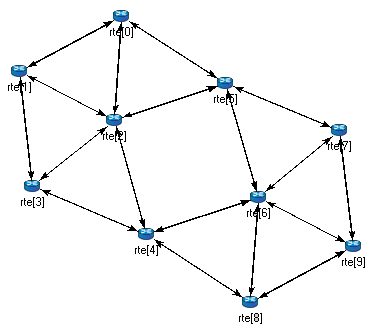
\includegraphics[scale=0.6]{figures/ned-routing-network}
    \caption{The network}
    \label{fig:ned-routing-network}
  \end{center}
\end{figure}

\begin{figure}[htbp]
  \begin{center}
    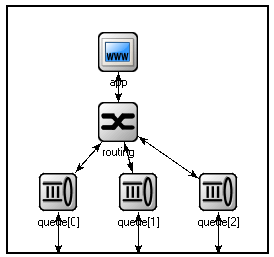
\includegraphics[scale=0.6]{figures/ned-routing-node}
    \caption{One node in the network}
    \label{fig:ned-routing-node}
  \end{center}
\end{figure}

Let us build the model bottom-up. First we define the simple module
types that will make up a network node. We need an application;
a module that performs network layer functions including routing;
and a module that queues up packets before they are transmitted on the
line. A NED file that declares them would look like this:

\begin{Verbatim}[commandchars=\\\{\}]
simple App
\{
    parameters:
        int address;  // local node address
        string destAddresses;  // destination addresses
        volatile double sendIaTime @unit(s) = default(exponential(1s));
                               // time between generating packets
        volatile int packetLength @unit(byte);  // length of one packet
        @display("i=block/browser");
    gates:
        input in;
        output out;
\}

simple Routing
\{
    parameters:
        @display("i=block/switch");
    gates:
        input in[];
        output out[];
        input localIn;
        output localOut;
\}

simple Queue
\{
    parameters:
        int frameCapacity = default(0); // max queue length; 0 means no limit
        @display("i=block/queue;q=queue");
    gates:
        input in;
        output out;
        inout line;
\}
\end{Verbatim}

It would also be possible (moreover, recommended) to put the above three
simple module declarations into separate \ttt{.ned} files: \ttt{App.ned},
\ttt{Routing.ned} and \ttt{Queue.ned}. Note that the NED language uses
the familiar curly brace syntax, and ``\ttt{//}'' to denote comments.

Let us see the first simple module type declaration. It declares a
\textit{module type} named \ttt{App}, which has four \textit{parameters}
called \ttt{address}, \ttt{destAddresses}, \ttt{sendIaTime} and \ttt{packetLength},
and also two \textit{gates} named \ttt{in} and \ttt{out}. The argument of
\ttt{@display()} is called a \textit{display string}, and it defines
the default rendering of the module in graphical environments;
\ttt{"i=..."} defines the default icon.

\begin{note}
    Note that the module type names (\ttt{App}, \ttt{Routing}, \ttt{Queue})
    begin with a capital letter, and parameter and gate names begin with
    lowercase -- this is the recommended naming convention. Capitalization
    matters because the language is case sensitive.
\end{note}

Notice that the declarations don't contain any code to define the operation
of the application (routing algorithm, queue) itself:
that part is expressed in C++. By default, {\opp} looks for a
C++ class of the same name (so here, \ttt{App}, \ttt{Routing} and {Queue}),
although this gets slightly more complicated if C++ namespaces or
NED packages are involved, and the user can also explicitly specify
which C++ class to use.

\ttt{App}'s parameters are of various data types (\ttt{int}, \ttt{double},
\ttt{string}) and some of them are also declared \ttt{volatile}. Parameters
can be read into C++ variables of similar types, and can be used by the
algorithm that drives the simple module. \ttt{volatile} practically means
that the parameter can be used as a source of random numbers.

\begin{note}
    With constructs like \ttt{exponential(1s)} assigned to the \ttt{sendIaTime}
    parameter in this example, \ttt{volatile} effectively means that
    there is no need to ever hardcode the distribution (e.g. "normal")
    into the C++ code, or to use multiple parameters to pass its mean,
    standard deviation etc into the C++ code. A single parameter can
    encapsulate all details, and can provide any random variable.
\end{note}

The \ttt{@unit(s)} and \ttt{@unit(byte)} bits declare the measurement unit
for the parameter. Values assigned to parameters must have the same or
compatible unit, i.e. \ttt{@unit(s)} accepts milliseconds, nanoseconds,
minutes, hours, etc., and \ttt{@unit(byte)} accepts kilobytes, megabytes,
etc. as well.

Generally, \ttt{@}-words like \ttt{@unit} and \ttt{@display} are called
\textit{properties} in NED, and they are used to annotate various objects
with metadata. Properties can be attached to parameters, gates, modules,
connections and other objects.

Both the \ttt{parameters:} and \ttt{gates:} sections in the simple module are
optional, that is, they can be left out if there's no parameter or gate.

Simple modules can be extended (or specialized) via subclassing. This will be
discussed in section \ref{sec:ch-ned-lang:inheritance}.

Comments in the NED source also serve a purpose in addition to making
the NED source more readable: in the {\opp} IDE they get displayed
at various places (tooltips, content assist, etc), and become part
of the documentation extracted from the NED files.
The NED documentation system, not unlike \textit{JavaDoc}
or \textit{Doxygen}, will be described in Chapter \ref{cha:neddoc}.

Now that we've learned enough about simple modules, we assemble our components
into a compound module type that represents a network node:

\begin{Verbatim}[commandchars=\\\{\}]
module Node
\{
    parameters:
        int address;
        @display("i=misc/node_vs,gold");
    gates:
        inout port[];
    submodules:
        app: App \{
            parameters:
                address = address;
                @display("p=140,60");
        \}
        routing: Routing \{
            parameters:
                @display("p=140,130");
            gates:
                in[sizeof(port)];
                out[sizeof(port)];
        \}
        queue[sizeof(port)]: Queue \{
            parameters:
                @display("p=80,200,row");
        \}
    connections:
        routing.localOut --> app.in;
        routing.localIn <-- app.out;
        for i=0..sizeof(port)-1 \{
            routing.out[i] --> queue[i].in;
            routing.in[i] <-- queue[i].out;
            queue[i].line <--> port[i];
        \}
\}
\end{Verbatim}

A compound module type, like simple modules, may have parameters and gates.
Our \ttt{Node} module contains an \ttt{address} parameter, plus a
\textit{gate vector} of unspecified size, named \ttt{port}.
The actual gate vector size will be determined implicitly by the number
of neighbours when we create a network from nodes of this type.
The type of \ttt{port[]} is \ttt{inout}, which basically means that
each gate is in fact a pair of gates, an input and an output gate;
they can also be addressed individually if needed, as \ttt{port\$i} and
\ttt{port\$o} (or rather, \ttt{port\$i[$k$]} and \ttt{port\$o[$k$]},
because now we have a gate vector.) Gate vectors can also be created with
a specified size, or be set to a fixed size at the place
of instantiating the module.

The point of compound modules is to serve as a container for other
modules. Our \ttt{Node} compound module type has an \ttt{app} and
a \ttt{routing} \textit{submodule}, plus a \ttt{queue[]} \textit{submodule vector}
that contains one \ttt{Queue} module for each port, as specified by
\ttt{[sizeof(port)]}.
Any module type (simple or compound module) can be used as a submodule.
Like simple modules, compound modules can also have gates and parameters,
and they can be used wherever simple modules can be used.

It is useful to think about compound modules as ``cardboard boxes''
that help you organize your simulation model and bring structure into
it. No active behaviour is associated with compound modules -- they
are simply meant for grouping modules into larger units that can
can be used either as a model (a \textit{network}, see later)
or as a building block for other compound modules.

Syntactically, a submodule may have a curly brace block as body, where
it is possible to assign its parameters (see \ttt{address} in the example),
set the size of gate vectors, or to add properties like the display string
(\ttt{@display}). Display strings specified here will be merged with the
display string from the type to get the effective display string.
The \ttt{"p="} tag used here means position on the canvas.

Connections are listed under the \ttt{connections} section of the
declaration. Not surprisingly, input and output gates are
connected with a normal arrow, and inout gates with a double-headed
arrow ``\ttt{<-->}''. Submodule vectors and gate vectors can be
connected with the familiar \ttt{for} syntax. Nesting and conditional
connections (\ttt{if}), although not shown here, are also possible.
Normally, NED checks that all gates be connected, but this can also
be turned off (\ttt{connections allowunconnected}).

All sections in a compound module declaration (\ttt{parameters},
\ttt{gates}, \ttt{submodules}, \ttt{connections}) are optional.

Now, we finally define the network, which consists of a few nodes that
are connected with lines:

\begin{Verbatim}[commandchars=\\\{\}]
network Net10
\{
    types:
        channel C extends ned.DatarateChannel \{
            parameters:
                delay = uniform(0.1ms, 1ms);
                datarate = 1Mbps;
        \}
    submodules:
        rte[10]: Node \{
            parameters:
                address = index;
        \}
    connections:
        rte[1].port++ <--> rte[0].port++;
        rte[0].port++ <--> rte[2].port++;
        rte[2].port++ <--> rte[5].port++;
        rte[5].port++ <--> rte[7].port++;
        rte[7].port++ <--> rte[9].port++;
        rte[9].port++ <--> rte[8].port++;
        rte[8].port++ <--> rte[4].port++;
        rte[4].port++ <--> rte[3].port++;
        rte[3].port++ <--> rte[1].port++;
        rte[3].port++ <--> rte[2].port++;
        rte[2].port++ <--> rte[4].port++;
        rte[4].port++ <--> rte[6].port++;
        rte[6].port++ <--> rte[8].port++;
        rte[9].port++ <--> rte[6].port++;
        rte[6].port++ <--> rte[7].port++;
        rte[5].port++ <--> rte[6].port++;
        rte[0].port++ <--> rte[5].port++;
        rte[1].port++ <--> rte[2].port++;
\}
\end{Verbatim}

There can be several network definitions in your NED file or NED files.
The simulation program that uses those NED files will be
able to run any of them; you typically select the desired one
in the config file (\ttt{omnetpp.ini}).

Naturally, only modules that have no gates can be a network.

A network is basically a compound module.

XXX channels, inner types, gate++

XXX add example ini file here!!!

XXX @isNetwork


%%% Local Variables:
%%% mode: latex
%%% TeX-master: "usman"
%%% End:



